\chapter{BUKTI KESALAHAN PEMILAHAN SAMPAH OLEH PENGGUNA}
\label{chap:lampiran-c}

Lampiran ini mendokumentasikan bukti visual kesalahan pemilahan sampah yang ditemukan selama periode observasi lapangan. Temuan ini menjadi dasar rekomendasi program sosialisasi pemilahan sampah pada Subbab \ref{sec:saran}.

\section*{C.1 Sampah Anorganik Dibuang ke Tempat Sampah Organik}

\begin{figure}[H]
  \label{fig:lamp-c1a}
  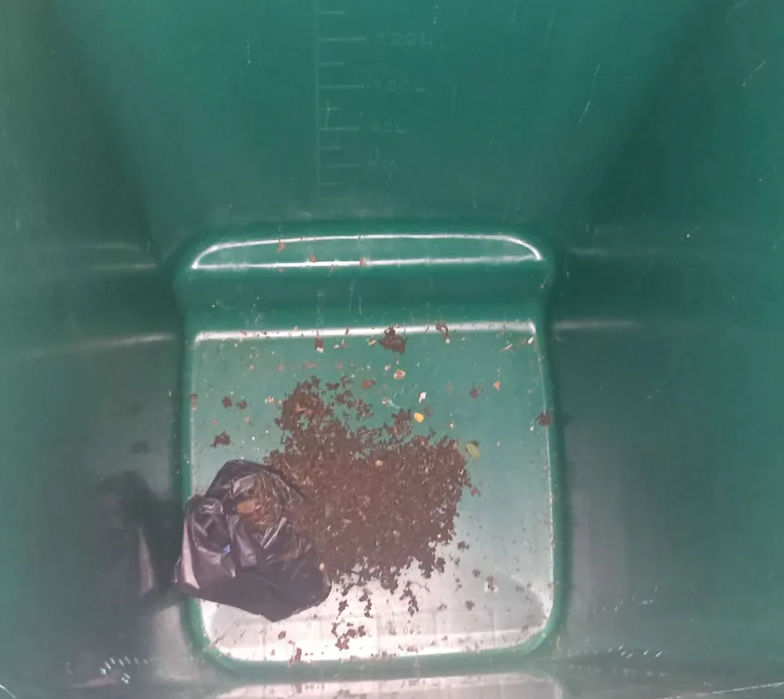
\includegraphics[width=0.75\textwidth]{images/salah-anorganik-ke-organik-1.png}
  \caption{Bukti 1: Sampah anorganik pada tempat sampah organik}
  % RENAME: image28.png → salah-anorganik-ke-organik-1.png
\end{figure}

\begin{figure}[H]
  \label{fig:lamp-c1b}
  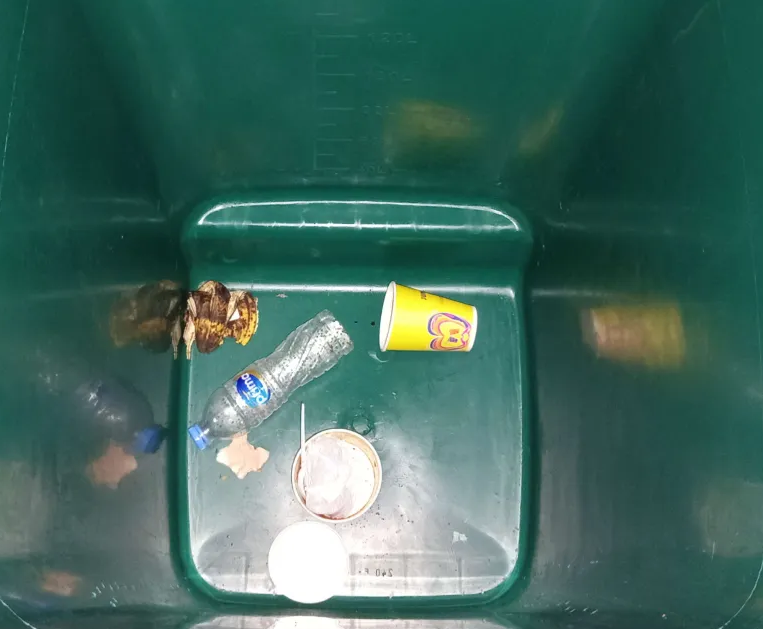
\includegraphics[width=0.75\textwidth]{images/salah-anorganik-ke-organik-2.png}
  \caption{Bukti 2: Sampah anorganik pada tempat sampah organik}
  % RENAME: image29.png → salah-anorganik-ke-organik-2.png
\end{figure}

\section*{C.2 Sampah Residu Dibuang ke Tempat Sampah Anorganik}

\begin{figure}[H]
  \label{fig:lamp-c2}
  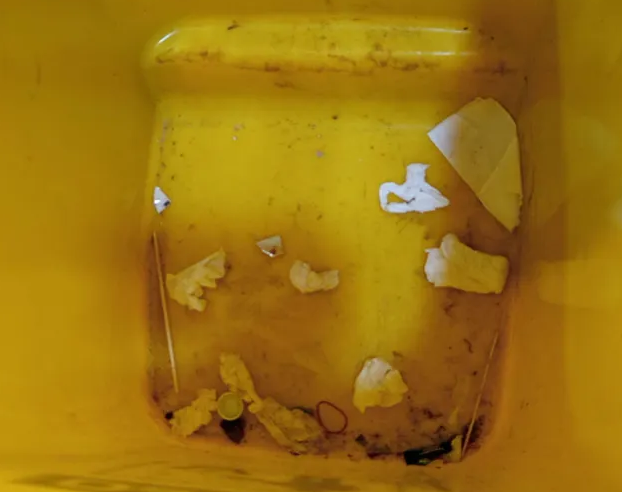
\includegraphics[width=0.65\textwidth]{images/salah-residu-ke-anorganik.png}
  \caption{Bukti: Sampah residu pada tempat sampah anorganik}
  % RENAME: image30.png → salah-residu-ke-anorganik.png
\end{figure}

\section*{C.3 Sampah Organik Dibuang ke Tempat Sampah Residu}

\begin{figure}[H]
  \label{fig:lamp-c3}
  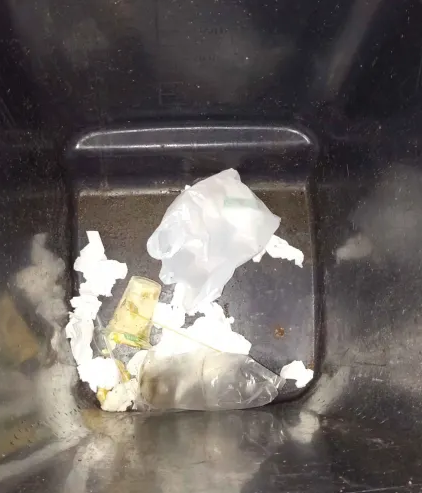
\includegraphics[width=0.75\textwidth]{images/salah-organik-ke-residu.png}
  \caption{Bukti: Sampah organik pada tempat sampah residu}
  % RENAME: image31.png → salah-organik-ke-residu.png
\end{figure}